    %----------------------------------------------------------------------------------------
%	PACKAGES AND THEMES
%----------------------------------------------------------------------------------------
\documentclass[aspectratio=169,xcolor=dvipsnames]{beamer}

\usepackage{hyperref}
\usepackage{graphicx} % Allows including images
\usepackage{booktabs} % Allows the use of \toprule, \midrule and \bottomrule in tables
\usepackage{bm}% bold math
\usepackage{physics}
\setlength{}{}%
\usepackage{siunitx}
\usepackage[inline]{asymptote}
\usepackage{multirow}
\usepackage{tikz}
\usepackage{pgfplots, pgfplotstable}
\usepackage{hyperref}
\usepackage{natbib}
% \usepackage{amsthm}
\usepackage{amssymb}
\usepackage{amsmath}
\usepackage{cancel}

\usepackage{xcolor} % more colors
\usetikzlibrary{positioning}
\tikzset{>=stealth}

\newcommand{\tikzmark}[3][]{\tikz[remember picture,baseline] \node [anchor=base,#1](#2) {$#3$};}

\definecolor{my-blue}{RGB}{93,169,233}
\definecolor{my-pink}{RGB}{238,118,116}
\definecolor{my-green}{RGB}{0,191,0}
\definecolor{my-orange}{HTML}{FE5F55}
\definecolor{background}{HTML}{f2f2f2}
\definecolor{my-yellow}{HTML}{F6BD60}
\definecolor{dark-blue}{HTML}{00008B}
\definecolor{my-maroon}{HTML}{800000}

\usepackage[breakable,many]{tcolorbox}
% Math

\tcbset{simple/.style={
            breakable,
            enhanced,
            outer arc=0pt,
            arc = 0pt,
            colback=background, % Background color
            colframe=background, % Border Color
            coltitle=black, % Title Color
            fonttitle=\bfseries,
            attach title to upper,
            after title={:\ },
            segmentation style={dashed, gray},
        }
}

\tcbset{color-labeled/.style={
            breakable,
            enhanced,
            outer arc=0pt,
            arc=0pt,
            colframe=#1,
            colback=#1!5,
            attach title to upper,
            coltitle=#1!200,
            after title={\medbreak},
        }
}

\tcbset{one-sided-color/.style={
            breakable,
            enhanced,
            boxrule=0pt,
            frame hidden,
            borderline west={2pt}{0pt}{#1},
            colback=#1!10,
            coltitle=#1!200,
            after title={:\ },
            sharp corners,
            attach title to upper,
        }
}

%%%%%%%%%%%%%%%%%%%%%%%%%%%%%%%%%%%%%%%%%%%%%%%%%%%%%%%%%%
%%%%%%%%%%%%%%%%%%   Box Definitions %%%%%%%%%%%%%%%%%%%%%
%%%%%%%%%%%%%%%%%%%%%%%%%%%%%%%%%%%%%%%%%%%%%%%%%%%%%%%%%%

\newtcolorbox[auto counter]{examplee}{
    simple,
    title=\textbf{Example} \thetcbcounter,
    % add a `\thetcbcounter` to the end if you want to keep track of numberings.
}

\newtcolorbox{mathematica}{
    simple,
    title=\textbf{Mathematica Snippet},
    % add a `\thetcbcounter` to the end if you want to keep track of numberings.
}

\newtcolorbox[auto counter]{experiment}{
    simple,
    title=\textbf{Experiment:},
    % add a `\thetcbcounter` to the end if you want to keep track of numberings.
}

\newtcolorbox[auto counter]{custom-big}[1][]{
    color-labeled=my-yellow,
    title=\textbf{{#1}},
}

\newtcolorbox{definitionn}{
    one-sided-color=my-green,
    title=\textbf{Definition},
}

\newtcolorbox{mnemonic}{
    one-sided-color=my-green,
    title=\textbf{Mnemonic},
}

\newtcolorbox{theoremm}{
    one-sided-color=my-blue,
    title=\textbf{Theorem},
}


\newtcolorbox[auto counter]{proposition}{
    one-sided-color=my-blue,
    title=\textbf{Proposition} \thetcbcounter,
}

\newtcolorbox[auto counter]{corollaryy}{
    one-sided-color=my-blue,
    title=\textbf{Corollary} \thetcbcounter,
}

\newtcolorbox[auto counter]{lemmaa}{
    one-sided-color=my-blue,
    title=\textbf{Lemma} \thetcbcounter,
}

% \newtcolorbox{proposition}{
%     one-sided-color=my-green,
%     title=\textbf{Proposition},
% }

%----------------------------------------------------------------------------------------
%	TITLE PAGE
%----------------------------------------------------------------------------------------

% The title
\title[short title]{Part II: The Hubbard Model and BCS Theory}
% \subtitle{Subtitle}

\author{QiLin Xue}
\institute[UofT] % Your institution may be shorthand to save space
{
    % Your institution for the title page
    University of Toronto
    \vskip 3pt
}
\date{\today} % Date, can be changed to a custom date


%----------------------------------------------------------------------------------------
%	PRESENTATION SLIDES
%----------------------------------------------------------------------------------------

\begin{document}

\begin{frame}
    % Print the title page as the first slide
    \titlepage
\end{frame}
%------------------------------------------------
\section{First Section}
%------------------------------------------------

\begin{frame}{Goal}
    \begin{itemize}
        \item Derive the theoretical relationship
        \begin{equation*}
            \frac{2|\Delta(T=0)|}{k_BT_c}=3.5278,
        \end{equation*}
        where $T_c$ is the critical temperature and $\Delta$ is the energy gap at $T=0.$
        \item Why is this interesting?
        \begin{itemize}
            \item Doesn't depend on material properties such as density of states, strength of electron interactions, etc.
            \item \textit{Universal}
        \end{itemize} 
    \end{itemize}
\end{frame}
\begin{frame}{Hubbard Model Hamiltonian}
    \begin{equation*}
        \hat{H} = \textcolor{red}{-t} \sum_{    
        \tikzmark{AAA}{\langle i,j\rangle},
        \sigma
        }(
        \tikzmark[red]{BBB}{\hat{c}^\dagger_{i\sigma}\hat{c}_{j\sigma} + \hat{c}^\dagger_{j\sigma}\hat{c}_{i\sigma}}
        )
        \textcolor{blue}{- U}\sum_i
        \tikzmark[blue]{CCC}{\hat{n}_{i\uparrow}\hat{n}_{i\downarrow}}
        % - \mu\sum_{i,\sigma}\hat{n}_{i\sigma},
    \end{equation*}

   \begin{tikzpicture}[overlay, remember picture,node distance =1.5cm]
        \node[,text width=3cm, yshift=1cm] (identitydescr) [below left=of AAA ]{look at all pairs of sites};
        \draw[,->,thick] (identitydescr) to [in=180,out=90] (AAA);


        \node[red, text width=4cm, yshift=1cm] (Gdescr) [below =of BBB]{creating electron at site $i$ and destroying electron at site $j$ (and vice-versa)};
        \draw[red,->,thick] (Gdescr) to [in=-90,out=90] (BBB);

        \node[blue,xshift=1.8cm,text width=4cm, yshift=1cm] (Ldescr) [below =of CCC]{attractive potential between electrons at the site $i$};
        \draw[blue,->,thick] (Ldescr) to [in=0,out=90] (CCC);
        % \node[purple,text width=2cm] (Cdescr) [below right =of C]{attenuation of the transmitted power};
        % \draw[purple,->,thick] (Cdescr) to [in=-90,out=90] (C.south);
    \end{tikzpicture}
    \vspace{8mm}
    \begin{center}
        \includegraphics[width=0.4\linewidth]{fig/2D-Hubbard-model.png}
    \end{center}
\end{frame}
\begin{frame}{The Partition Function}
    The Partition function is given by 
    \begin{equation*}
        Z = \text{Tr}(e^{-\beta\hat{H}})
    \end{equation*}
    After a lot of tedious mathematics, we get 
    \begin{equation*}
        Z = \int \exp\left(- \underbrace{\int_0^\beta \left[\sum_{i}\bar{c}_{i\tau}\partial_\tau c_{i\tau} + H[\bar{c}, c]\right] \dd{\tau}}_{\text{The Action } S}\right) \mathcal{D}\bar{c} \mathcal{D}c
    \end{equation*} 
\end{frame}
\begin{frame}{The Hubbard-Stratonovich Transformation}
    We can write 
    \begin{equation*}
        e^{Un_{\uparrow}n_{\downarrow}} = e^{U\bar{c}_{\uparrow}\bar{c}_{\downarrow}c_{\downarrow}c_{\uparrow}} = \int \exp\left(-\frac{1}{U}|\Delta(T=0)|^2 - \Delta \bar{c}_\uparrow \bar{c}_\downarrow - \Delta^* c_{\downarrow}c_{\uparrow} \right)\dd{\Delta^*}\dd{\Delta}.
    \end{equation*}
    We can rewrite the action in terms of $\Delta,\Delta^*.$ If $Z=\int e^{-S_\text{eff}} \mathcal{D}\Delta^* \mathcal{D}\Delta$ then
    \begin{equation*}
        S_\text{eff} = \int_0^\beta \underbrace{\sum_i \frac{1}{U}|\Delta_{i\tau}|^2}_{\text{gaussian term}} \dd{\tau} - \underbrace{\log \left\langle \exp\left(-\int_0^\beta \sum_i (\Delta_{i\tau}\bar{c}_{i\tau\uparrow}\bar{c}_{i\tau\downarrow} + h.c.) \dd{\tau}\right)\right\rangle_0}_{\text{interaction term (between cooper pairs)}}
    \end{equation*}
    We write the interaction term as 
    \begin{equation*}
        \Delta S_\text{eff} = -\log \langle e^{-S'}\rangle_0
    \end{equation*}
\end{frame}
\begin{frame}{Cumulant Expansion}
    Recall that 
    \begin{align*}
        e^x &= 1 + x + \frac{x^2}{2} + \frac{x^3}{3!} + \cdots \\ 
        \log(1+x) &= x - \frac{x^2}{2} + \frac{x^3}{3} + \cdots
    \end{align*}
    Then:
    \begin{align*}
        -\log( \langle e^{-S'} \rangle_0) &= -\log(1 + \langle {-S'}\rangle_0  + \frac{1}{2} \left\langle\left({S'}\right)^2 \right\rangle_0 + \cdots ) \\ 
        &= \langle S' \rangle_0 + \frac{1}{2} \left\langle S'^2 \right\rangle_0 - \frac{1}{2}\langle S' \rangle_0^2 + \cdots
    \end{align*}
    We will compute up to order 2.
\end{frame}
\begin{frame}{Cumulant Expansion}
    We wish to compute 
    \begin{equation*}
        \Delta S_\text{eff} \approx \langle S' \rangle_0 + \frac{1}{2} \left\langle S'^2 \right\rangle_0 - \frac{1}{2}\langle S' \rangle_0^2
    \end{equation*}
    We compute
    \begin{equation*}
        \langle S'\rangle_0 = \langle \bar{c}_{k-p,\uparrow},\bar{c}_{p,\downarrow} \rangle_0 = 0.
    \end{equation*}
    and
    \begin{equation*}
        \frac{1}{2} \langle S'^2\rangle_0 = -\frac{1}{\beta N}\sum_k |\Delta_k|^2 \pi(\bm{k},ik_0)
    \end{equation*}
\end{frame}
\begin{frame}{Effective Action}
    We derived 
    \begin{equation*}
        S_\text{eff} = \frac{1}{\beta N}\sum_k |\Delta_k|^2\left(\frac{1}{U} - \pi(\bm{k},ik_0)\right)
    \end{equation*}
    A transition occurs when the coefficient of $|\Delta_k|^2$ changes sign. Can analytically determine when $\bm{k}=k_0=0.$ We get from complex analysis, 
    \begin{equation*}
        \pi(0,0) = \rho \log\left(\frac{2\beta D}{\pi}e^\gamma\right)
    \end{equation*}
    Gives a formula for the critical temperature
    \begin{equation*}
        \boxed{T_c \sim \frac{2De^\gamma}{\pi k_B}e^{-1/({\rho}U)}}
    \end{equation*}
\end{frame}
\begin{frame}{The Big Picture}
    \begin{center}
        \begin{tikzpicture}
        \begin{axis}[
        legend pos=outer north east,
        title=Phase Transition,
        axis lines = middle,
        xticklabels={},
        yticklabels={},
        xlabel = $T$,
        ylabel = $\Delta$,
        variable = t,
        trig format plots = rad,
        ]
        \addplot [
            domain=0:1.75,
            samples=70,
            color=blue,
            ]
            {sqrt(1.75-x)};
        \end{axis}
        \end{tikzpicture}
    \end{center}
\end{frame}
\begin{frame}{Some More Assumptions}
    \begin{itemize}
        \item $\Delta$ is a constant in space and time.
        \item $D \gg |\Delta(T=0)|$
        \item $\rho(\xi) = \begin{cases}
            \rho_0 & |\xi| < D \\ 
            0 & \text{else}
        \end{cases}$
        \item Analytically analyze as $T \to 0$ (at the very end)
    \end{itemize}
    \begin{center}
        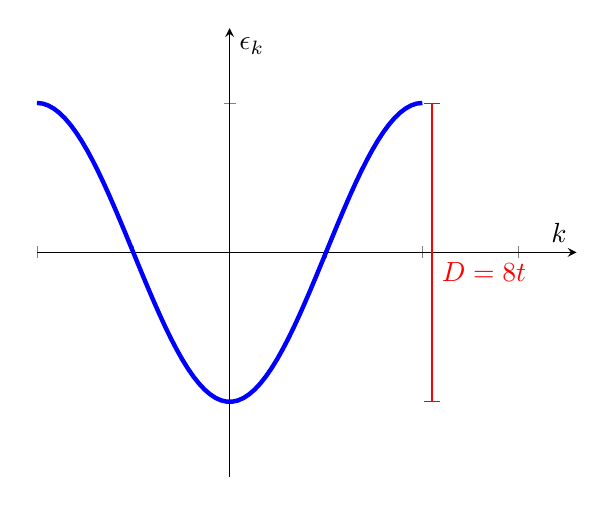
\begin{tikzpicture}
            \begin{axis}[
                axis lines = middle,
                xlabel = $k$,
                ylabel = {$\epsilon_k$},
                xticklabels={},
                yticklabels={},
                xmin=-10,
                xmax=18,
                ymin=-1.5,
                ymax=1.5,
                trig format plots = rad,
            ]
            \addplot[blue, ultra thick, samples=70, domain=-10:10] {-cos((pi/10)*x)};
            \draw[|-|,yshift=0,red] (axis cs: 10.5,1) -- node[below right] {$D=8t$} (axis cs: 10.5,-1);
            \end{axis}
            \end{tikzpicture}
    \end{center}


\end{frame}
\begin{frame}{Action Minimization}
    Going back a bit... The action (as a functional)
    \begin{equation*}
        S_\text{eff}[\Delta^*,\Delta] = \int_0^\beta \underbrace{\sum_i \frac{1}{U}|\Delta_{i\tau}|^2}_{\text{gaussian term}} \dd{\tau} - \underbrace{\log \left\langle \exp\left(-\int_0^\beta \sum_i (\Delta_{i\tau}\bar{c}_{i\tau\uparrow}\bar{c}_{i\tau\downarrow} + h.c.) \dd{\tau}\right)\right\rangle_0}_{\text{interaction term}}
    \end{equation*}
    becomes a regular function,
    \begin{equation*}
        S_\text{eff}(\Delta^*,\Delta) =  \frac{\beta N |\Delta(T=0)|^2}{U} - \log \left\langle \exp\left(-\int_0^\beta \sum_i (\Delta \bar{c}_{i\tau\uparrow}\bar{c}_{i\tau\downarrow} + h.c.) \dd{\tau}\right)\right\rangle_0
    \end{equation*}
    which we can minimize with respect to $\Delta^*$ which gives
    \begin{equation*}
        \Delta = - \frac{U}{\beta N}\sum_k \langle c_{-k,\downarrow}c_{k,\uparrow}\rangle
    \end{equation*}
\end{frame}
\begin{frame}{Diagonalization}
    Assuming $\Delta$ is constant allows us to write the action as 
    \begin{equation*}
        S_\text{eff}(\Delta^*,\Delta) = \frac{\beta N|\Delta(T=0)|^2}{U} + \sum_{\bm{k},\omega} \begin{pmatrix}\bar{c}_{k,\uparrow} & c_{-k,\downarrow}
        \end{pmatrix}\begin{pmatrix}
            -i\omega + \xi_{\bm{k}} & \Delta \\ 
            \Delta^* & -i\omega - \xi_{\bm{k}}
        \end{pmatrix}\begin{pmatrix}
            c_{k,\uparrow} \\ \bar{c}_{-k,\downarrow}
        \end{pmatrix}
    \end{equation*}
    We can diagonalize this, using the action minimization condition, and the assumptions above, after (a lot of) work, we get 
    \begin{equation*}
        |\Delta(T=0)| = 2De^{-1/\rho U}
    \end{equation*}
\end{frame}
\begin{frame}{Finishing Up}
    We have 
    \begin{align*}
        T_c = \frac{2De^\gamma}{\pi k_B}e^{-1/(\rho U)},\qquad |\Delta(T=0)| = 2De^{-1/\rho U}
    \end{align*}
    so dividing through, we get 
    \begin{equation*}
        \frac{2|\Delta(T=0)|}{k_BT_c} = 2\pi e^{-\gamma} = 3.5278
    \end{equation*}
    \begin{center}
        \includegraphics[width=0.5\linewidth]{fig/table.png}
    \end{center}
\end{frame}
\end{document}